
\cleardoublepage
\appendix

% --- Start Appendix (A, B, C, ...) ---
\setcounter{chapter}{0}
\renewcommand{\thechapter}{\Alph{chapter}}
\renewcommand{\thesection}{\thechapter.\arabic{section}}
\renewcommand{\thesubsection}{\thesection.\arabic{subsection}}
\renewcommand{\thesubsubsection}{\thesubsection.\arabic{subsubsection}}

% --- Hyperref: unique link anchors ---
\renewcommand{\theHchapter}{app.\Alph{chapter}}
\renewcommand{\theHsection}{\theHchapter.\arabic{section}}
\renewcommand{\theHsubsection}{\theHsection.\arabic{subsection}}
\renewcommand{\theHsubsubsection}{\theHsubsection.\arabic{subsubsection}}

\chapter{Mathematical Background and Derivations}
\label{anhangA}

This appendix presents the mathematical and physical concepts discussed in the main text
in a more formal and detailed way. The goal is to avoid overloading the didactic readability
of the chapters while still giving interested readers
access to the complete derivations.

% ============================================================
\section{Derivation of the Irrationality of $\sqrt{2}$}
\label{anhangA_wurzel2}

\subsection*{The Irrationality of \texorpdfstring{$\sqrt{2}$}{sqrt(2)}}

The proof that $\sqrt{2}$ is irrational is one of the oldest and
most elegant proofs by contradiction\index{proof by contradiction} in mathematics.
The idea is simple: we assume that $\sqrt{2}$ is rational and then
show that this assumption leads to a logical contradiction.

\subsubsection*{Assumption}

We assume that $\sqrt{2}$ can be written as a fully reduced fraction
\[
\sqrt{2} = \frac{p}{q},
\]
where $p$ and $q$ are integers,
$q \neq 0$, and $p$ and $q$ are relatively prime.

\subsubsection*{Squaring}

Squaring both sides gives
\[
2 = \frac{p^2}{q^2}
\qquad\Rightarrow\qquad
p^2 = 2q^2.
\]

The right-hand side is even, so $p^2$ must also be even.
Therefore $p$ itself is even. Thus there is an integer $r$ such that
\[
p = 2r.
\]

\subsubsection*{Substitution and a Second Conclusion}

Substituting this into the equation $p^2 = 2q^2$, we obtain
\[
(2r)^2 = 2q^2,
\]
hence
\[
4r^2 = 2q^2.
\]

Dividing by $2$ gives
\[
2r^2 = q^2.
\]

So $q^2$ is also even -- and therefore $q$ itself is even.

\subsubsection*{The Contradiction}
\index{contradiction}

We have now shown:
\[
p \text{ is even}, \qquad q \text{ is even}.
\]
Thus $p$ and $q$ have the common factor $2$ and are not
relatively prime.

This contradicts our initial assumption that $\frac{p}{q}$ was fully
reduced.

\subsubsection*{Conclusion}

The assumption that $\sqrt{2}$ is rational therefore leads to a contradiction.
Hence
\[
\sqrt{2} \text{ is irrational.}
\]

In its basic form, this classical proof already goes back to Euclid\index{Euclid}
and shows impressively how proofs by contradiction work.

\begin{DidacticBox}[Why This Proof Is So Elegant]
	\phantomsection\label{box:proof-elegant}
	The proof of the irrationality of $\sqrt{2}$ is a classical
	example of how powerful proofs by contradiction can be.
	From an apparently harmless assumption, a logical impossibility follows.
	Thus the proof shows not only that $\sqrt{2}$ is irrational,
	but also how precise mathematical thinking works.
\end{DidacticBox}

% ============================================================
\section{Construction of the Complex Numbers}
\label{anhangA_komplexe}
\index{complex numbers}

The necessity of complex numbers arises from a simple
problem: some equations have no solution in the real numbers.
A particularly clear example is
\[
x^2 + 1 = 0.
\]

Rearranging gives
\[
x^2 = -1.
\]

But no real number has a negative square.
Here, therefore, a limit of the real number system becomes visible.
Nevertheless, such expressions inevitably occur
when solving certain equations -- for example in the \emph{casus irreducibilis}\index{casus irreducibilis}
of cubic equations.

\subsubsection*{A New Type of Number}

To make the equation $x^2 = -1$ solvable, one introduces a new number
and defines
\[
i := \sqrt{-1}.
\]
\index{imaginary unit $i$}

This definition is not a mere trick, but a genuine extension
of the number system: we extend the real numbers so that equations
with negative squares can also be solved meaningfully.

\subsubsection*{The Structure of the New Number Type}

Every number of the form
\[
a + bi, \qquad a,b \in \mathbb{R},
\]
\index{complex number $a+bi$}
is called a \emph{complex number}. The familiar rules of arithmetic remain valid;
the only new piece of information is
\[
i^2 = -1.
\]

From this, addition and multiplication are completely determined.
For example:
\[
(2 + 3i)(4 - i)
= 8 - 2i + 12i - 3i^2
= 11 + 10i.
\]

\begin{DidacticBox}[Why the Introduction of $i$ Is Necessary]
	\phantomsection\label{box:i-necessary}
	The number $i$ is not introduced because one wanted to ``invent'' it.
	It arises from the inner logic of algebra.
	Once one accepts the rules of calculation for equations,
	the equation
	$x^2 = -1$
	forces the introduction of a new type of number.
	
	All complex numbers then follow from the minimal assumption
	$i^2 = -1$.
	This completes the number system:
	every nonconstant polynomial now has at least one root
	(Fundamental Theorem of Algebra).\index{Fundamental Theorem of Algebra}
\end{DidacticBox}

\subsubsection*{Euler's Formula as a Geometric Addition}
\index{Euler's formula}

The introduction of the number $i$ opens not only a new number domain,
but also connects the exponential function with circular motion.
This is shown by the famous Euler formula
\[
e^{i\varphi} = \cos\varphi + i\sin\varphi.
\]

\subsubsection*{Brief Derivation of Euler's Formula Using Taylor Series}
\index{Taylor series}

Euler's formula
\[
e^{i\varphi} = \cos\varphi + i\sin\varphi
\]
can be derived elegantly using power series.

First, we consider the series expansions of the functions
$e^x$, $\cos x$, and $\sin x$ around the point $x=0$:
\begin{align*}
	e^x &= 1 + x + \frac{x^2}{2!} + \frac{x^3}{3!} + \frac{x^4}{4!} + \cdots,\\[1ex]
	\cos x &= 1 - \frac{x^2}{2!} + \frac{x^4}{4!} - \frac{x^6}{6!} + \cdots,\\[1ex]
	\sin x &= x - \frac{x^3}{3!} + \frac{x^5}{5!} - \frac{x^7}{7!} + \cdots.
\end{align*}

Now substitute $x = i\varphi$ into the exponential series:
\[
e^{i\varphi} = 1 + i\varphi + \frac{(i\varphi)^2}{2!}
+ \frac{(i\varphi)^3}{3!}
+ \frac{(i\varphi)^4}{4!}
+ \cdots.
\]

Using the powers of $i$,
\[
i^2 = -1,\quad i^3 = -i,\quad i^4 = 1,\quad i^5 = i,\;\dots,
\]
we can sort the terms. We separate the real and imaginary parts:

\begin{align*}
	e^{i\varphi}
	&= \Bigl(1 - \frac{\varphi^2}{2!} + \frac{\varphi^4}{4!} - \frac{\varphi^6}{6!} + \cdots\Bigr)
	\;+\; i\Bigl(\varphi - \frac{\varphi^3}{3!} + \frac{\varphi^5}{5!} - \frac{\varphi^7}{7!} + \cdots\Bigr)\\[1ex]
	&= \cos\varphi + i\sin\varphi.
\end{align*}

Thus Euler's formula
\[
e^{i\varphi} = \cos\varphi + i\sin\varphi
\]
is derived as a direct consequence of the series expansions of the exponential,
sine, and cosine functions.

\subsubsection*{Geometric Idea}

If one considers the complex plane, a point on the
unit circle\index{unit circle} describes an angle $\varphi$ with the real axis.
The projection onto the two axes gives
\[
(\cos\varphi,\;\sin\varphi).
\]
\index{sine}
\index{cosine}

Since the imaginary axis is interpreted as a multiple of $i$,
this point corresponds to the complex number
\[
\cos\varphi + i\sin\varphi.
\]

Euler's formula shows that the complex exponential function
describes exactly this circular motion on the unit circle.

\begin{center}
	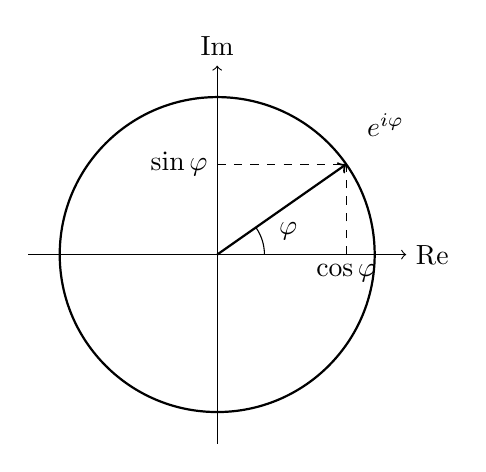
\begin{tikzpicture}[scale=2]
		% Circle
		\draw[thick] (0,0) circle (1);
		% Axes
		\draw[->] (-1.2,0) -- (1.2,0) node[right] {Re};
		\draw[->] (0,-1.2) -- (0,1.2) node[above] {Im};
		% Angle
		\draw[thick,->] (0,0) -- ({cos(35)},{sin(35)});
		\draw (0.3,0) arc (0:35:0.3);
		\node at (0.45,0.15) {$\varphi$};
		% Projections
		\draw[dashed] ({cos(35)},0) -- ({cos(35)},{sin(35)});
		\draw[dashed] (0,{sin(35)}) -- ({cos(35)},{sin(35)});
		% Labels
		\node[below] at ({cos(35)},0) {$\cos\varphi$};
		\node[left] at (0,{sin(35)}) {$\sin\varphi$};
		\node at ({cos(35)+0.25},{sin(35)+0.25}) {$e^{i\varphi}$};
	\end{tikzpicture}
\end{center}

\subsubsection*{Multiplication by \boldmath$i$ as Rotation}
\index{rotation (multiplication by $i$)}

In the complex plane, multiplication by $i$ has a simple geometric
meaning: it rotates every number by $90^\circ$ counterclockwise.

Examples:
\[
1 \xrightarrow{\;\cdot i\;} i \xrightarrow{\;\cdot i\;} -1
\xrightarrow{\;\cdot i\;} -i \xrightarrow{\;\cdot i\;} 1
\]

Each further multiplication by $i$ adds another rotation by $90^\circ$.
The important point is: the absolute value remains unchanged -- only the direction changes.

The exponential function $e^{i\varphi}$ combines infinitely many such
small rotations. This creates a continuous rotation on the
unit circle whose angle is exactly $\varphi$.

\subsubsection*{Why Multiplication by \boldmath$i$ Produces a Rotation}

Let us consider a point on the unit circle:
\[
e^{i\varphi} = \cos\varphi + i\sin\varphi.
\]

If we multiply this point by $i$, we obtain
\[
i \cdot e^{i\varphi}
= i(\cos\varphi + i\sin\varphi)
= i\cos\varphi - \sin\varphi.
\]

This corresponds to the new complex number
\[
-\sin\varphi + i\cos\varphi.
\]

That is exactly what one obtains by rotating the original point
\((\cos\varphi,\;\sin\varphi)\)
by \(90^\circ\) counterclockwise:
\[
(\cos\varphi,\;\sin\varphi)
\;\longrightarrow\;
(-\sin\varphi,\;\cos\varphi).
\]

Thus it is clear:
\[
i \cdot e^{i\varphi}
\]
is exactly the point rotated by \(90^\circ\) -- with unchanged radius.

\begin{DidacticBox}[Core Idea of Euler's Formula]
	\phantomsection\label{box:euler-coreidea}
	Multiplication by $i$ means a rotation by $90^\circ$ in the complex plane.
	The exponential function $e^{i\varphi}$ combines many such small rotations
	into a single rotation through the angle $\varphi$.
	
	Therefore:
	\[
	e^{i\varphi} = \cos\varphi + i\sin\varphi.
	\]
\end{DidacticBox}

\subsubsection*{Conclusion}

Complex numbers extend the real numbers by exactly what is missing
to treat algebraic equations completely.
From the single specification $i^2=-1$, a complete number domain arises
with clear rules of calculation and an intuitive geometric structure.

% ============================================================
\section{Mandelbrot Map: Mathematical Generation and Coloring}
\label{app:mandelbrot-rendering}

\index{Mandelbrot set}
\index{iteration}
\index{escape radius}
\index{escape time}
\index{parameter space}
\index{complex plane}
\index{coloring}
\index{algorithm}

\textbf{Purpose of this appendix:} This section shows how a typical Mandelbrot graphic is generated algorithmically:
from the image pixel to the parameter \(c\), then to the escape time, and finally to the color assignment.

\begin{MathBox}[Basic Principle: Pixel \(\rightarrow\) Parameter \(c\) \(\rightarrow\) Iteration]
	\phantomsection\label{box:mandelbrot-basic-principle}
	For each image point, we compute a parameter \(c\in\mathbb{C}\) and iterate
	\[
	z_{n+1}=z_n^2+c,\qquad z_0=0.
	\]
	The Mandelbrot set is the set of parameters \(c\) for which the sequence \(\{z_n\}\) remains bounded.
\end{MathBox}

\subsection{Coordinate Transformation: From Pixel to the Complex Plane}
\index{coordinate transformation}

Let an image have width \(W\) and height \(H\). We choose a viewing window
\[
x\in[x_{\min},x_{\max}],\qquad y\in[y_{\min},y_{\max}]
\]
and assign to each pixel \((i,j)\) (with \(0\le i<W\), \(0\le j<H\)) a parameter \(c=x+iy\):
\[
x(i)=x_{\min}+\frac{i}{W-1}\,(x_{\max}-x_{\min}),\qquad
y(j)=y_{\max}-\frac{j}{H-1}\,(y_{\max}-y_{\min}),
\]
\[
c(i,j)=x(i)+i\,y(j).
\]
The minus sign in \(y(j)\) appears because image coordinates typically increase downward.

\begin{NoteBox}[Typical Standard Window]
	\phantomsection\label{box:mandelbrot-standard-window}
	A commonly used viewing window is
	\[
	x\in[-2.5,1.0],\qquad y\in[-1.2,1.2].
	\]
	For detail views or zooms, one chooses a smaller window around a center \(c_0\).
\end{NoteBox}

\subsection{Escape-Time Algorithm: Escape Criterion and Iteration Number}
\index{escape criterion}

For each \(c\), we iterate up to a maximum number \(N_{\max}\). As soon as \(|z_n|>R\), we stop.
For the Mandelbrot iteration, the classical choice \(R=2\) is sufficient:

\begin{MathBox}[Escape Radius \(R=2\)]
	\phantomsection\label{box:mandelbrot-escape-radius}
	For \(z_{n+1}=z_n^2+c\), the following holds: if for some \(n\), \(|z_n|>2\), then the sequence certainly diverges.
\end{MathBox}

Formally, we define the \textbf{escape time}
\[
n_\text{esc}(c)=\min\{n\in\mathbb{N}\mid |z_n|>2\},
\]
if it exists; otherwise we set \(n_\text{esc}(c)=N_{\max}\) and mark the point as ``inside'' -- typically black.

\subsection{Coloring: Discrete, Smooth, and Intuitive}
\index{color scale}

\subsubsection{(a) Discrete Coloring by Escape Time}

The simplest method: assign color only according to \(n_\text{esc}\).
This often leads to visible ``bands,'' but it is didactically very clear.

\subsubsection{(b) Smooth Coloring / Continuous Coloring}

To avoid banding, one uses a \textbf{continuous} iteration count. A common variant is:
\[
\nu(c)=n + 1 - \log_2\!\bigl(\log |z_n|\bigr),
\]
where \(n\) is the first index with \(|z_n|>2\). Here \(\nu\) lies between \(n\) and \(n+1\).

\begin{DidacticBox}[Why This ``Log-Log'' Formula?]
	\phantomsection\label{box:mandelbrot-loglog}
	Outside the set, \(|z_n|\) grows approximately quadratically.
	The expression \(\log(\log(\cdot))\) rescales this growth
	so that color gradients become smooth and the structure near the boundary becomes much more visible.
\end{DidacticBox}

From \(\nu\), one then forms a number \(t\in[0,1]\) -- for example by scaling -- and passes \(t\) through a color palette.

\subsubsection{(c) Histogram Equalization (optional)}

More advanced renderings count how many pixels have which escape time, form a cumulative distribution, and distribute colors so
that frequent values do not ``clump together.'' This yields very balanced images, but it is a display technique, not the mathematics of the set itself.

\subsection{Pseudocode: Compact and Transparent}
\index{pseudocode}

\begin{verbatim}
	Input: W,H, x_min,x_max, y_min,y_max, N_max, R=2
	for j = 0..H-1:
	y = y_max - j*(y_max-y_min)/(H-1)
	for i = 0..W-1:
	x = x_min + i*(x_max-x_min)/(W-1)
	c = x + I*y
	z = 0
	n = 0
	while n < N_max and |z| <= R:
	z = z*z + c
	n = n + 1
	if n == N_max:
	color(i,j) = black
	else:
	nu = n + 1 - log2(log(|z|))
	color(i,j) = palette(nu)
	Output: PNG image
\end{verbatim}

\begin{NoteBox}[Important Note for the Reader]
	\phantomsection\label{box:mandelbrot-reader-note}
	The Mandelbrot set itself is mathematically determined only by the distinction
	\emph{inside} vs.\ \emph{outside}, that is, by
	\emph{bounded} vs.\ \emph{divergent}.
	Everything else -- color palette, smoothing, histogram methods --
	belongs to visualization technique, not to the definition of the set itself.
\end{NoteBox}

% ============================================================
\section{From Minimal Length to Minimal Surface: Optimal Branching Networks}
\label{app:netzwerke-minimalflaeche}
\index{optimization}
\index{minimal surface}
\index{network}
\index{branching}
\index{transport network}

In the main text, a modern method transfer was discussed:
biological structures such as neurons, blood vessels, or trees are not ideal ``wires,''
but tube networks with finite thickness.
This also changes the natural objective function of the optimization:
not only total length is relevant, but above all the required surface area
as well as the geometric cost of branching points.

\subsection{The 1D Model: Minimizing Total Length}
\index{graph}
\index{Steiner tree}

A network is modeled as a graph: nodes are branching points or endpoints, and edges $e$ are connections with length $\ell_e$.
A natural minimal principle is:
\begin{equation}
	K_{\text{L}} = \sum_{e} \ell_e.
	\label{eq:cost_length}
\end{equation}
This model is suitable for systems in which ``material'' is proportional to length and branches are treated as ideal points.
In mathematics, this leads toward the Steiner problem: one seeks a network that connects given endpoints with minimal total length.

\medskip
\noindent
\textbf{Limit of the 1D model.}
As soon as connections have finite thickness, a pure length functional becomes too crude:
a ``cable'' is then no longer one-dimensional, but has a lateral surface that must be built and maintained.

\subsection{The 2D Model: Tube Surface Instead of Length}
\index{cylinder}
\index{surface area}

An edge $e$ is approximated as a cylinder with radius $r_e$ and length $\ell_e$.
Then the lateral surface area is
\begin{equation}
	A_e \approx 2\pi r_e\, \ell_e,
	\qquad
	A \approx \sum_e 2\pi r_e\, \ell_e.
	\label{eq:area_sum}
\end{equation}
Here, ``area'' means the sum of the lateral surface areas of the tube segments as a cost measure,
not a connected minimal surface as in the case of a soap film.

If surface area represents the cost of material, membrane, maintenance, or stability, then a simple cost function is
\begin{equation}
	K_{\text{A}} = \alpha \sum_e r_e\, \ell_e.
	\label{eq:cost_area}
\end{equation}
Here $\alpha>0$ is a weighting factor that fixes units and scaling and, in applications,
can summarize additional effects.
\index{minimal surface}
\begin{MathBox}[From Wire to Tube: The Decisive Step]
	\phantomsection\label{box:wire-tube}
	
	The 1D model minimizes length $\sum \ell_e$.
	The 2D model takes thickness into account and minimizes surface costs proportional to
	$\sum r_e\ell_e$.
	This turns a \emph{line problem} into a \emph{surface problem}:
	the geometry of branches is determined not only by ``shortest paths,''
	but by ``the smoothest possible structure with low surface area.''
\end{MathBox}

\subsection{Branches Are Not Free: Junction Costs}
\index{junction}
\index{curvature}

In real networks, a branch is not an ideal point operation.
Geometrically, local curvatures, transition regions, and mechanical stresses arise;
functionally, regulation, stability, and fault tolerance are added.
This can be modeled by an additional term:
\begin{equation}
	K = \alpha \sum_e r_e\,\ell_e \;+\; J\,N_{\text{J}},
	\label{eq:cost_with_junctions}
\end{equation}
where $N_{\text{J}}$ is the number of junctions and $J>0$ is a ``junction penalty.''

\paragraph{Mini-example: trifurcation vs.\ two bifurcations.}
\index{trifurcation}
\index{bifurcation}

Three endpoints are to be supplied. Two plausible designs:
\begin{itemize}
	\item \textbf{Design A:} one three-way branch, or one junction, with total length $L_A$.
	\item \textbf{Design B:} two two-way branches, or two junctions, with total length $L_B$.
\end{itemize}
For constant radius, the comparison
\[
K_A \approx \alpha L_A + J,
\qquad
K_B \approx \alpha L_B + 2J.
\]
is sufficient.
Design A is cheaper if
\begin{equation}
	\alpha(L_A-L_B) < J.
	\label{eq:threshold_J}
\end{equation}

\textbf{Interpretation:}
Even if Design A is somewhat longer, it can be optimal as soon as the junction is ``expensive enough.''
The threshold is $J/\alpha$: only when the junction is more expensive than the saved effective length
does the additional branch no longer pay off.

\subsection{Transport Costs as a Second Mechanism}
\index{Poiseuille's law}
\index{flow resistance}

Surface area is not everything: a network transports flow, such as water, blood, or signals.
For laminar flow in a cylindrical tube, the flow resistance scales approximately as
$R \sim \ell/r^4$.
This leads to another plausible cost component:
\begin{equation}
	K_{\text{T}} = \beta \sum_e \frac{\ell_e}{r_e^4},
	\label{eq:transport_cost}
\end{equation}
where $\beta>0$ describes the weighting of transport losses.
A combined model is then:
\begin{equation}
	K = \alpha \sum_e r_e\,\ell_e \;+\;
	\beta \sum_e \frac{\ell_e}{r_e^4}
	\;+\; J\,N_{\text{J}}.
	\label{eq:full_cost}
\end{equation}

\textbf{Interpretation:}
\begin{itemize}
	\item Larger radii reduce transport losses, but are more expensive in terms of surface area and material.
	\item Additional branches can distribute flow, but produce junction costs.
\end{itemize}

Exactly such conflicts of objectives generate the typical, strikingly optimized branching architectures in nature.
\index{string theory}
\begin{DidacticBox}[Key Point: Not Strings in the Brain -- But Surface Optimization]
	\phantomsection\label{box:stringtheory-surfaceoptimization}
	The connection to string theory is \emph{methodological}, not ontological:
	many problems can be formulated as the minimization of a surface functional.
	In modern physics, powerful mathematical tools have been developed for this.
	Here they are used to describe real branching networks as optimization problems.
\end{DidacticBox}

\subsection{Conclusion}
\index{mathematics}

The central step is the change of model:
from ``shortest lines'' to ``low-surface tubes with branching cost.''
This makes understandable why nature, in many contexts
-- for example in trees, vessels, or neurons --
leads to similar geometries.
Not because the systems are identical, but because their optimization logic is structurally related.

% ============================================================
\section{The Fibonacci Sequence and the \newline  Golden Ratio}
\label{app:fibonacci-goldener-schnitt}

The Fibonacci sequence is a recursively defined sequence of numbers.
It begins with
\[
F_1 = 1,\qquad F_2 = 1
\]
and each further number is obtained as the sum of the two preceding numbers:
\[
F_{n+2} = F_{n+1} + F_n \qquad (n \geq 1).
\]

The first terms are therefore:
\[
1,\;1,\;2,\;3,\;5,\;8,\;13,\;21,\;34,\dots
\]

What is mathematically especially interesting is that the ratios of two consecutive Fibonacci numbers
\[
\frac{F_{n+1}}{F_n}
\]
approach, as \(n\) grows, a fixed number, namely the \emph{golden ratio}
\[
\varphi = \frac{1+\sqrt{5}}{2} \approx 1{,}618.
\]

Thus:
\[
\lim_{n\to\infty} \frac{F_{n+1}}{F_n} = \varphi.
\]

This connection is significant for many growth and arrangement problems.
In plants, Fibonacci numbers do not appear because a plant ``calculates,''
but because certain rules of space distribution and growth lead to spiral structures
in which such numbers often occur.